
\documentclass{report}

%% Packages for French writing
\usepackage[francais]{babel}
\usepackage[utf8]{inputenc}
\usepackage[T1]{fontenc}
\usepackage{layout}

%% Packages for Math symbols
\usepackage[fleqn]{amsmath}
\usepackage{amssymb}
\usepackage{mathrsfs}

%% Packages for figures insertion
\usepackage{graphicx}
\usepackage{wrapfig}
\usepackage{framed}
\usepackage{float}

%% Package for document margin editing
\usepackage[top=2cm, bottom=2cm, left=2cm, right=2cm]{geometry}

%% Package for source code insertion
\usepackage{listings}
\usepackage{xcolor}
\definecolor{grey}{rgb}{0.97, 0.97, 0.97}
\definecolor{darkred}{rgb}{0.42, 0, 0}
\definecolor{darkblue}{rgb}{0, 0, 0.42}
\definecolor{darkgrey}{rgb}{0.22, 0.22, 0.82}
\definecolor{green}{HTML}{088A08}
\lstset{
  basicstyle=\small\sffamily\footnotesize,
  captionpos=b,
  numbers=left,
  numberstyle=\tiny,
  tabsize=4,
  frame=trBL,
  backgroundcolor=\color{grey},
  commentstyle=\color{green},
  keywordstyle=\color{darkblue}\bf,
  identifierstyle=\color{darkgrey},
  stringstyle=\color{darkred}
}

\title{Rapport de projet VLSI}
\author{Nicolas Phan, Kevin Mambu}
\date{pour le 26 Janvier 2018}
\begin{document}
\pagestyle{headings}
\maketitle
\tableofcontents

%==================================================================================================
%=========================  Introduction  =========================================================
%==================================================================================================
\section{Introduction}

%----------------- Objectif -----------------------------------------------------------------------
\subsection{Objectif}

Le but de notre projet est de concevoir un processeur ARM, c'est à dire un processeur conforme
à l'architecture décrite dans la documentation ARM donnée en cahier des charges.

%----------------- Processus de developpement -----------------------------------------------------
\subsection{Processus de développement}

La conception de ce processeur se fera en quatre grandes étapes :

\begin{figure}[h]
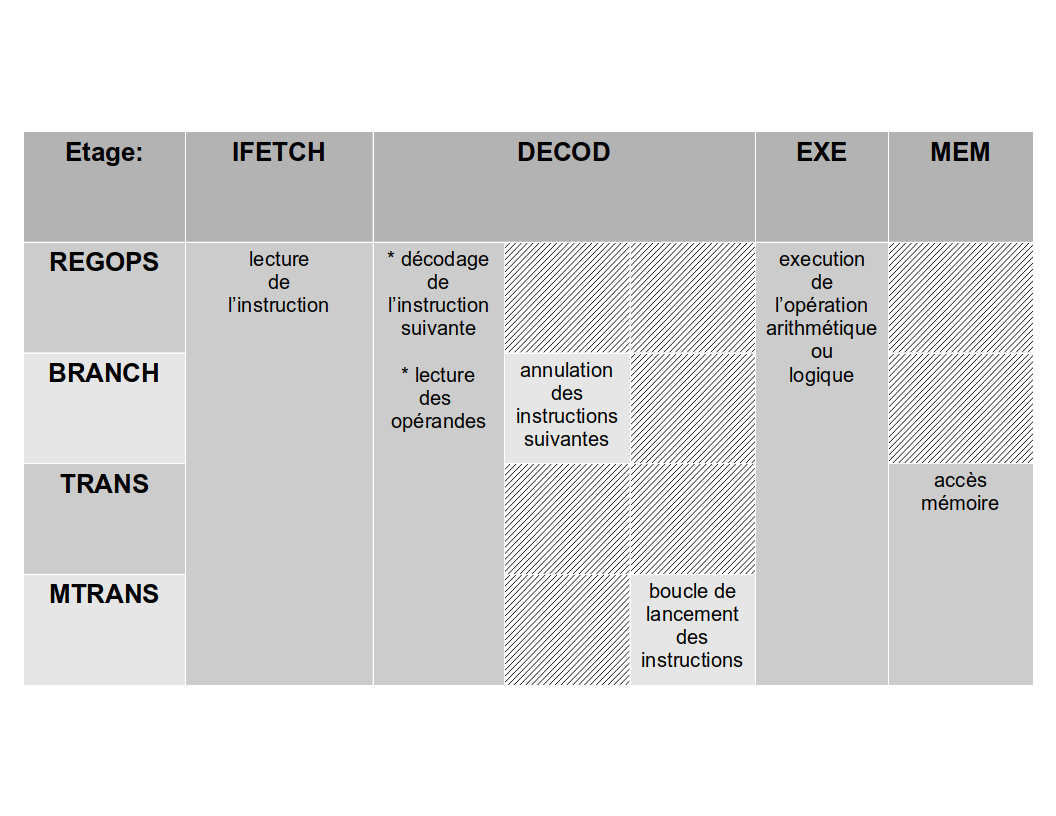
\includegraphics[scale=1]{pics/blank.png}
\centering
\caption{Schema-bloc des étapes de conception du processeur} 
\end{figure}

\begin{enumerate}
\item \textbf{Modélisation}  : Cela consiste en la description d'un modèle du processeur,
                      la description peut avoir différents niveaux d'abstraction
                      du plus abstrait (description du comportement du circuit seulement)
                      au plus concret (schema des portes logiques du circuit)
                      \textit{Nous utiliserons le langage VHDL pour décrire notre modèle de processeur}
\item \textbf{Simulation}    : Il s'agit de simuler notre processeur.
                      \textit{Nous utiliserons le simulateur ghdl ainsi que des bancs de tests VHDL
                      et une plateforme de simulation d'exécution de programmes ASM et C}
\item \textbf{Placement, Routage} : Dans cette étape, nous passons d'un modèle VHDL du circuit à un
                          dessin du masque de notre processeur, prêt à être envoyé en fonderie.
                          \textit{Nous utiliserons les outils druc, cougar, lvx, tas et s2r pour cela}
\item \textbf{Fonderie} :          Cette étape est réalisée par un fondeur tiers.
\end{enumerate}

%==================================================================================================
%=========================  Modelisation  =========================================================
%==================================================================================================
\section{Modélisation}

\subsection{Design général du processeur}

Le processeur doit pouvoir exécuter toutes les instruction du jeu ARM avec le moins
de matériel possible, de plus, nous devrons concevoir un processeur pipeliné asynchrone.
La figure \ref{etages} illustre le découpage en étages de notre pipeline avec les opérations effectuées
par chaque étage pour chaque type d'instruction.
Les types d'instructions que nous étudierons seront les instructions de data processing (regops),
les instructions de branchement (branch), les transferts mémoires simples (trans) et multiples (mtrans).

\begin{figure}[h]
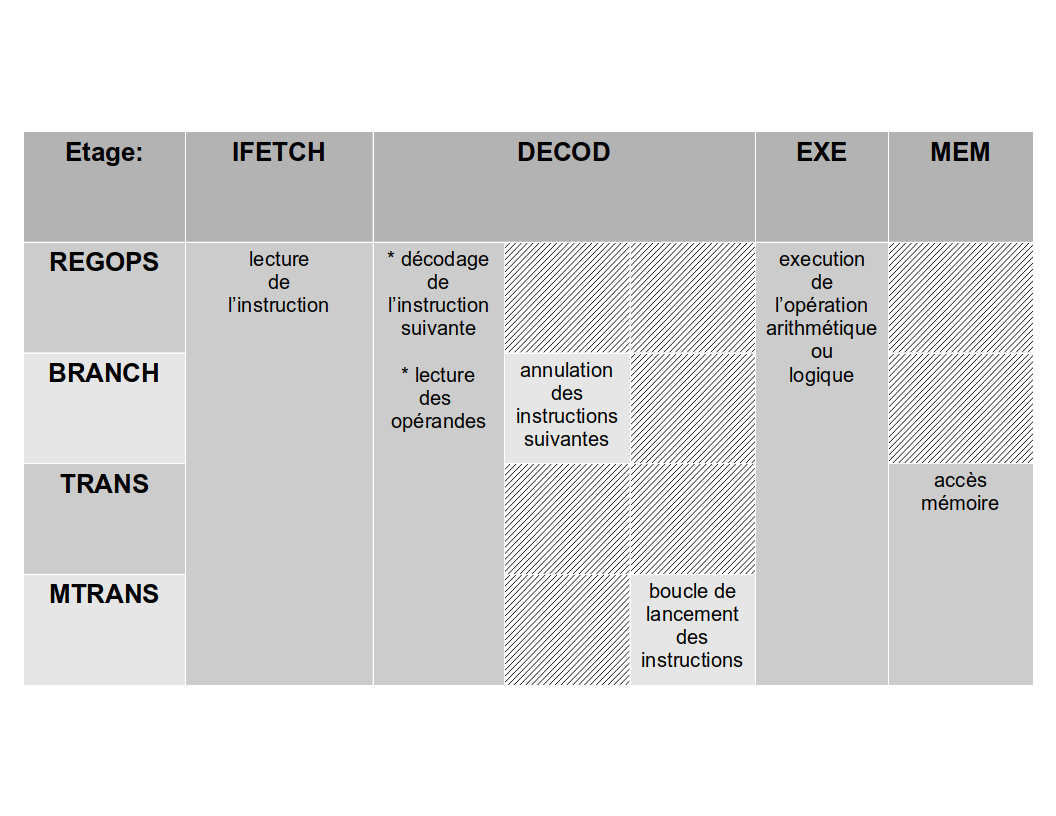
\includegraphics[scale=1]{pics/blank.png}
\centering
\caption{Découpage en étages du processeur}
\label{etages}
\end{figure}

\subsection{Modélisation de l'étage EXE}

C'est à l'étage EXE que se feront les opérations de calcul lors de l'execution d'instructions,
cela comprend le calcul de l'adresse destination lors d'un branchement.
Pour concevoir cet étage, nous devons nous demander quelles sont tous les calculs possibles
que l'étage devra pouvoir réaliser.

Les différents types d'instructions que nous avons sont les regops, les branch, les trans et mtrans,
or les branch, trans et mtrans n'ont besoin d'effectuer que des additions (pour le calcul d'adresses
mémoire) et les regops contiennent une instruction d'addition, donc si l'étage EXE peut effectuer
les calculs nécéssaires aux regops, a fortiori il couvre aussi les branch et transferts mémoire.
Cela réduit le problème au cas des regops.

Il faut lister l'ensemble des calculs que EXE devra effectuer et les réécrire
de manière standardisée pour les décomposer en un sous-ensemble de calculs élémentaires.
Cela nous permettra de trouver une implémentation de EXE réduisant au maximum le matériel nécéssaire.

\begin{figure}[h]
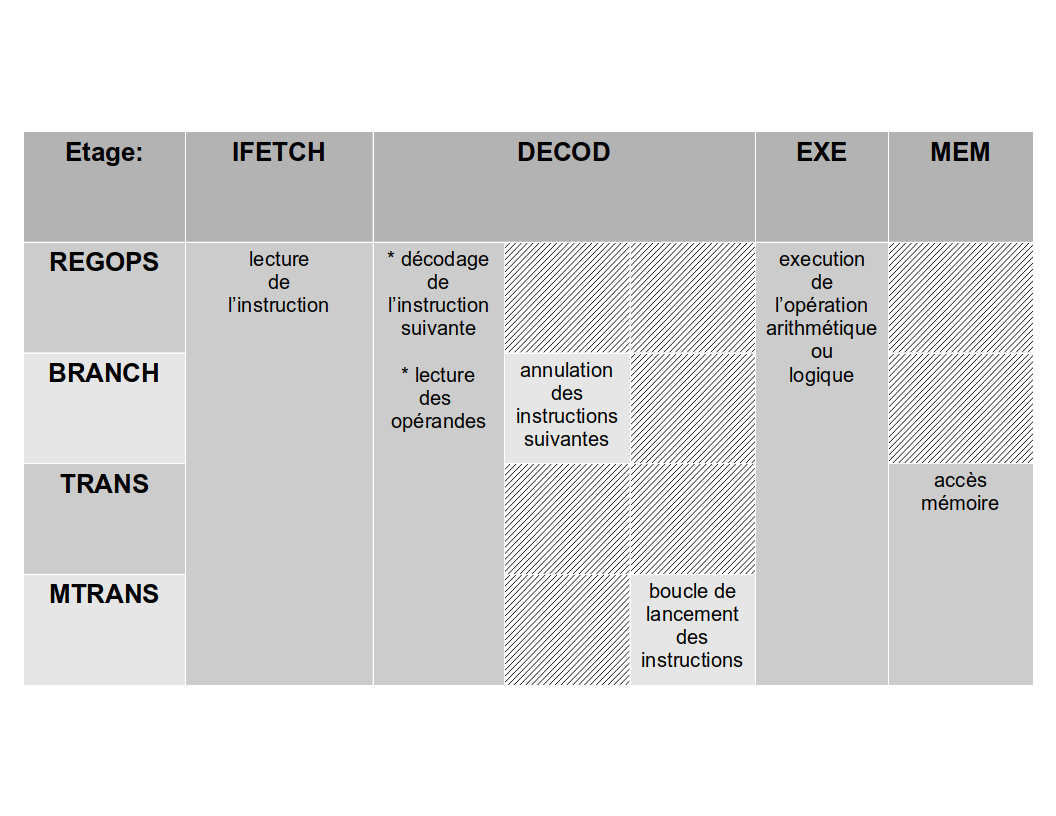
\includegraphics[scale=1]{pics/blank.png}
\centering
\caption{Standardisation des calculs demandés par les regops}
\label{standard}
\end{figure}

On peut voir sur la figure \ref{standard} que l'ensemble des calculs demandés se décompose
en calculs élémentaires suivants :
\begin{itemize}
  \item ADD, AND, OR, XOR
  \item Inversion des entrées au préalable
  \item Ajout d'un 1 pour l'additino (retenue en entrée)
\end{itemize}

De plus, le jeu d'instruction ARM spécife que l'opérande 1 peut subir un décalage
parmi 5 types (lsl, lsr, asr, ror, rrx) et qu'à chaque opération, les flags de sortie
doivent être calculés, on a donc :
\begin{itemize}
  \item Décalage de l'opérande 1
  \item Calcul des flags de sortie
\end{itemize}

Avec tous ces éléments, nous aboutissons au schema Figure \ref{exe} pour EXE.

\begin{figure}[h]
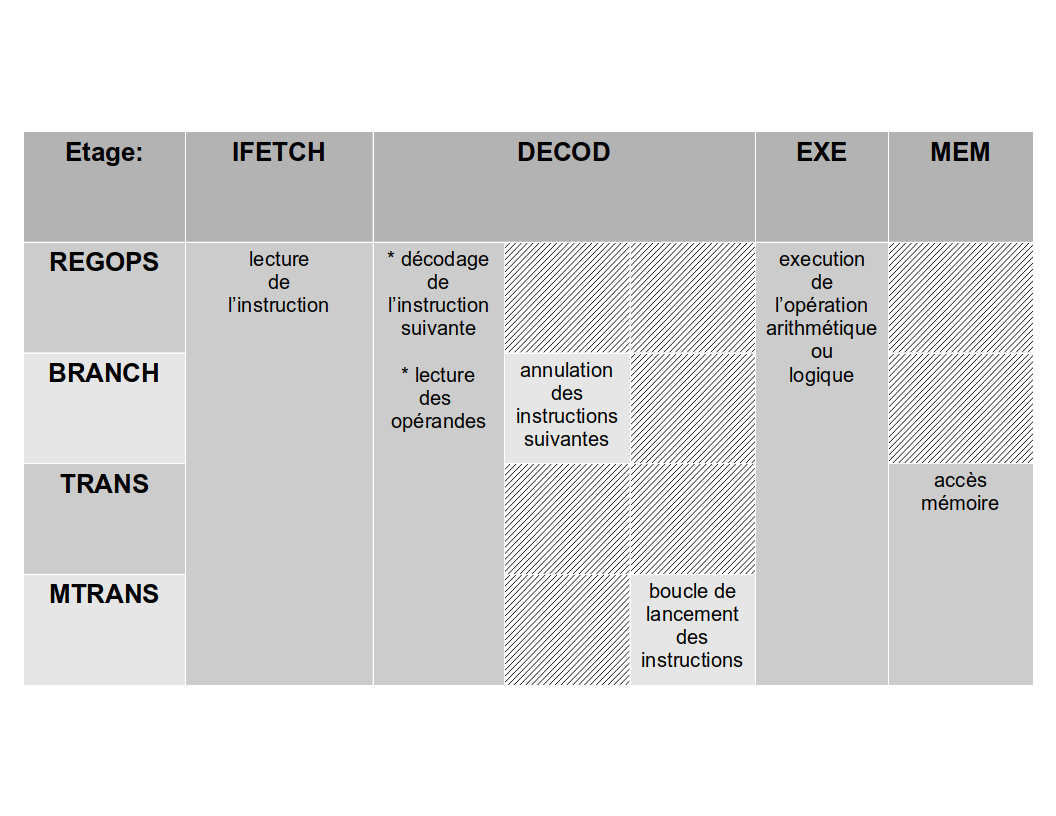
\includegraphics[scale=1]{pics/blank.png}
\centering
\caption{Schema de l'étage EXE}
\label{exe}
\end{figure}


%==================================================================================================
%=========================  End of the Document  ==================================================
%==================================================================================================

\end{document}
